% ---------------------------------------------------%
% DISCLAIMER: ADA KEMUNGKINAN BAB 3 STRUKTUR YG DIBAHAS BERBEDA, JADI DI BAWAH ADA CONTOH
% BAB 3 KATING. MODIF SAJA SESUAI KEBUTUHAN

% ---------------------------------------------------%

% \chapter{Analisis dan Perancangan}
\chapter{Analisis Masalah dan Solusi}

\section{Analisis Masalah}

Protokol komunikasi pada dasarnya dibangun untuk melayani komunikasi data antara dua buah pihak yang berbeda. Hal ini sesuai syarat jaringan komputer yang telah dijelaskan pada bagian II.1. Protokol komunikasi harus dapat memastikan pesan yang dikirimkan dapat diterima oleh pihak penerima pesan serta dipahami isinya. Selain itu, protokol komunikasi juga harus memastikan ancaman apabila terdapat pihak ketiga yang terlibat baik secara aktif ataupun pasif. Oleh karena itu, terdapat beberapa permasalahan yang akan dibahas pada bagian ini.

\subsection{Analisis Kebutuhan Protokol Komunikasi Rahasia}

Dalam jaringan komunikasi, pesan yang dikirimkan dapat mengalami kegagalan. Hal ini dapat menyebabkan pesan yang dikirimkan tidak diterima oleh pihak penerima. Dengan asumsi protokol ini berdiri di atas jaringan yang reliabel, kegagalan yang mungkin terjadi diantaranya adalah adanya kerusakan pada algoritma pengiriman, terjadi kerusakan pada perangkat, ataupun ada pihak ketiga yang terlibat secara aktif pada jaringan. Hal ini dapat menyebabkan \emph{frame} yang dikirimkan dianggap valid oleh layer dibawahnya, tetapi pada layer protokol ini dianggap tidak valid. Oleh karena itu, perlu adanya sebuah mekanisme untuk menangani kegagalan pengiriman pesan.

Dalam mengirimkan pesan, terdapat ancaman dari pihak ketiga yang terlibat secara aktif maupun pasif. Hal ini dapat terjadi dikarenakan pesan dikirimkan melalui jalur komunikasi yang tidak aman. Oleh karena itu, terdapat beberapa ancaman keamanan yang ada pada protokol komunikasi yang dibangun. Ancaman ini akan dibahas lebih lanjut pada bagian selanjutnya.

Protokol yang dibangun akan memanfaatkan sistem \emph{chaos} sebagai pembangkitan kunci blok dan kunci MAC. Hal ini memerlukan sebuah mekanisme agar sistem pembangkitan kunci dapat tersinkronisasi melalui mekanisme \emph{handshake} pada TLS. 

Pada protokol TLS, kunci MAC yang digunakan dalam beberapa cipher suite bersifat statis. Hal ini dapat mengancam komunikasi dikarenakan dapat membuat \emph{state} dari salah satu pihak tidak sesuai. Hal ini memerlukan analisis lebih lanjut terkait metode pembaharuan kunci TLS sehingga komunikasi tetap dapat berjalan dengan baik walaupun terdapat serangan terhadap sistem MAC ini.

Pada protokol TLS berbasis chaos, kunci blok yang digunakan bersifat dinamis. Hal ini memerlukan analisis lebih lanjut terkait metode pembaharuan kunci blok yang digunakan pada protokol ini pada masing-masing pihak. Hal ini diperlukan agar \emph{state} dari kunci blok dapat terjamin.

\subsection{Ancaman Keamanan pada Protokol Komunikasi}

Pada bagian sebelumnya, telah dijelaskan bahwa terdapat pihak ketiga yang mungkin terlibat dalam komunikasi. Hal ini dapat menimbulkan beberapa ancaman keamanan yang ada pada protokol komunikasi yang dibangun. Bagian ini akan menjelaskan rincian analisis ancaman keamanan yang dihadapi oleh protokol ini. Untuk mempermudah penjelasan, diasumsikan terdapat dua buah pihak yang melakukan komunikasi, yaitu Ahmad dan Budi. Terdapat pihak ketiga dalam komunikasi bernama Candra sebagai pihak yang tidak berhak terlibat dalam komunikasi. 

Dalam komunikasi, memungkinkan Candra mengaku sebagai salah satu pihak yang terlibat dalam komunikasi, yaitu Ahmad dan Budi. Hal ini dapat dilakukan dengan melakukan serangan MITM di antara kedua belah pihak. Dengan melakukan serangan ini, memungkinkan Candra mendapatkan informasi yang dikirimkan oleh Ahmad dan Budi. Oleh karena itu, perlu adanya mekanisme untuk memastikan bahwa pihak yang terlibat merupakan pihak yang dipercaya.

Selain itu, Candra juga dapat melakukan serangan berupa \emph{replay attack}. Dalam serangan ini, Candra bertujuan untuk mengganggu sistem dengan mengirimkan ulang pesan-pesan tertentu yang telah direkam. Candra mungkin tidak dapat mengetahui isi dari data yang ada pada \emph{frame}, tetapi \emph{frame} tersebut dapat menyebabkan efek yang tidak diinginkan oleh Ahmad ataupun Budi. Oleh karena itu, perlu adanya otentikasi partisipan pada pesan.

Dalam komunikasi, Candra dapat mengubah \emph{frame} yang dikirimkan oleh Ahmad ataupun Budi. Hal ini dapat menyebabkan pesan yang dikirimkan tidak dapat dipahami oleh penerima. Selain itu, hal ini dapat memberikan efek yang tidak diinginkan oleh penerima, seperti \emph{bitflip} attack. Oleh karena itu, perlu adanya mekanisme untuk menjaga integritas pesan yang dikirimkan oleh Ahmad ataupun Budi.

Dalam proses komunikasi, salah satu pihak yang terlibat baik Ahmad maupun Budi dapat menyangkal telah mengirimkan sebuah \emph{frame} dalam komunikasi. Untuk mengcegah hal tersebut, diperlukan sebuah mekanisme nirpenyangkalan dari tiap-tiap peserta yang telah mengirimkan pesan.

Pesan yang dikirimkan dalam jaringan publik dapat diamati oleh Candra. Candra dapat mengetahui isi pesan terenkripsi yang telah dikirimkan oleh Ahmad ataupun Budi. Hal ini dapat dicapai dengan melakukan beberapa teknik diantaranya adalah melakukan \emph{brute force} terhadap kunci enkripsi. Teknik lainnya yang dapat dilakukan oleh Candra adalah melakukan analisis kunci enkripsi. Salah satu teknik yang bisa dilakukan adalah melakukan analisis berbasikan \emph{plaintext} yang telah diketahui. Candra dapat mengamati pola yang dibentuk dari hasil enkripsi. Candra juga dapat melakukan analisis terhadap \emph{ciphertext} yang telah diterima. Hal ini dapat dilakukan dengan melakukan analisis frekuensi terhadap blok pesan ataupun melakukan analisis secara visual terhadap \emph{ciphertext}. Harapan dari proses ini mendapatkan pola dari \emph{ciphertext} sehingga dapat dianalisis apa isi pesan yang terenkripsi.

Pada jaringan komunikasi publik, Candra dapat membanjiri pesan tidak bermakna dengan ukuran cukup besar kepada salah satu pihak, misalkan Budi. Hal ini dapat menyebabkan Budi akan sibuk untuk melakukan dekripsi pesan besar dan tidak dapat menerima pesan dari Ahmad. Oleh karena itu, diperlukan otentikasi pengirim pesan agar dapat dipastikan pesan yang dilakukan dekripsi merupakan pihak yang berhak.

\section{Analisis Solusi}

Bagian ini akan menjelaskan terkait solusi dari permaslahan yang telah dipaparkan sebelumnya. Bagian ini akan dibagi menjadi beberapa kategori, diantaranya adalah solusi terkait dengan proses sistem chaos, sinkronisasi sistem chaos, proses enkripsi dan dekripsi, dan proses otentikasi pengirim pesan.

\subsection{Sistem Chaos}

Pada penelitian yang dilakukan oleh \textcite{lin2021}, sistem chaos yang digunakan adalah sistem chaos berbasis Hénon Map. Nilai hasil pembangkitan diambil melalui parameter $X_n$ yang dihasilkan pada setiap iterasi. Bila diamati melalui persamaan \ref{eq:chaos.henon}, bila diketahui nilai $X_n$, akan sangat sulit untuk mendapatkan nilai $X_{n-1}$ dikarenakan diperlukannya nilai $Y_n$ yang tidak diketahui. Oleh karena itu, sistem chaos ini sukar untuk mendapatkan nilai mundur. Kelemahan dari sistem \emph{chaos} ini adalah distribusi yang tidak \emph{uniform}. Hal ini dapat dilihat pada gambar \ref{fig:chaos.henon.distribution}.

\begin{figure}[!h]
  \centering
  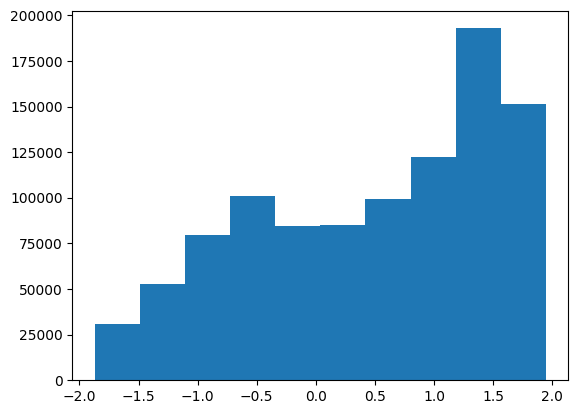
\includegraphics[width=250px]{chapters/res/chapter-3/img/henon.distribution.png}
  \caption{Distribusi nilai dari sistem chaos Hénon Map dengan $a=1$ dan $b=0.1$} \label{fig:chaos.henon.distribution}
\end{figure}

Hal ini dapat diperbaiki dengan melibatkan sistem chaos berbasis \emph{sine map}. Sistem chaos berbasis \emph{sine map} dipilih dikarenakan sistem chaos ini menghasilkan titik diantara $0$ dan $1$ sehingga memudahkan dalam melakukan konversi dalam byte.

Dalam perpaduan dua sistem \emph{chaos} ini masih memiliki kekurangan. Hal ini dikarenakan apabila seseorang mengetahui dua buah nilai berturut-turut dari sistem \emph{chaos}, nilai \emph{chaos} selanjutnya dapat diprediksi. Untuk mengatasi hal tersebut, dapat dilibatkan sistem \emph{chaos} berbasis sinus map untuk dilibatkan sebagai pengganggu parameter kedua. Pada sistem pengganggu ini, digunakannya sistem logistik dikarenakan saat melakukan \emph{inverse} dari sistem ini, memerlukan ketelitian sangat tinggi untuk mendapatkan nilai sebelumnya yang benar. Hal ini dapat mempersulit proses untuk mendapatkan nilai c yang benar. % TODO: Cari alasan yang lebih bener!!!

Dari hasil tersebut, dapat dibentuk sistem \emph{chaos} yang didefinisikan pada persamaan \ref{eq:tls.chaos}.

\begin{equation}
  \begin{aligned}
    X_{i+1} = \text{mod}((1 - a \cdot X_i^2 + Y_i) + (\frac{\mu}{4} \cdot \sin{(\pi \cdot X_{i})}) \cdot 100, 1)  \\
    Y_{i+1} = \text{mod}((b \cdot X_i + Z_{i}) \cdot 100, 1) \\
    Z_{i+1} = \frac{\mu}{4} \cdot \sin{(\pi \cdot Z_{i})}
  \end{aligned}
  \label{eq:tls.chaos}
\end{equation}

Pada persamaan \ref{eq:tls.chaos}, terdapat pengali dengan nilai $100$. Nilai ini digunakan untuk memperoleh distribusi hasil yang lebih baik lagi. Selain itu, nilai pengali ini ditujukan untuk mengacak nilai pecahan yang dihasilkan untuk nilai-nilai yang baru.

\subsection{Sinkronisasi Sistem Chaos}

Menurut \textcite{lin2021}, sinkronisasi sistem \emph{chaos} dapat dilakukan dengan memanfaatkan \emph{sliding mode control}. Namun, metode ini memerlukan RTT yang cukup banyak untuk melakukan sinkronisasi. Pada protokol TLS, pada dasarnya telah disediakan mekanisme untuk pertukaran kunci dengan melalui proses \emph{handshake}. Oleh karena itu, sinkronisasi sistem \emph{chaos} dapat dilakukan dengan memanfaatkan \emph{master key} dari proses tersebut.

Permasalahan selanjutnya adalah terkait dengan konversi nilai \emph{master key} menjadi nilai \emph{state} pada sistem \emph{chaos}. Prasayat dari sistem \emph{chaos} pada persamaan \ref{eq:tls.chaos} adalah nilai $X_0$, $Y_0$, dan $Z_0$ harus berada pada range $(0,1)$. Oleh karena itu, proses konversi dapat dilakukan dengan menghitung perbandingan nilai pada blok hasil ekspansi kunci dengan nilai maksimum blok tersebut. Hal ini dinyatakan pada persamaan \ref{eq:tls.convert}.

\begin{equation}
  \begin{aligned}
    f(K) = \frac{K}{2^{n}} \\
  \end{aligned}
  \label{eq:tls.convert}
\end{equation}

Dalam hal ini nilai $n$ adalah jumlah bit maksimum. Pada protokol yang dibangun, jumlah bit yang diambil adalah $n = 256$. Hal ini didasari dengan tipe data float memiliki ketelitian yang cukup baik pada 32 bit.

\subsection{Enkripsi dan Dekripsi Pesan}

Pada saat proses enkripsi ataupun dekripsi pesan, diperlukan bit-bit kunci yang dibangkitkan melalui sistem \emph{chaos}. Proses pengubahan titik \emph{chaos} pada persamaan \ref{eq:tls.chaos} menjadi bilangan bulat dapat dilakukan persamaan \ref{eq:tls.convert.int}.

\begin{equation}
  \begin{aligned}
    K_i = \lfloor{X_i \cdot 2^{n}}\rfloor
  \end{aligned}
  \label{eq:tls.convert.int}
\end{equation}

Proses pengubahan ini diambil dikarenakan $K_i$ yang dihasilkan akan langsung berada pada jumlah bit yang dibutuhkan. Hal ini dapat menghemat operasi yang diperlukan dalam melakukan konversi.

Permasalahan selanjutnya adalah terkait dengan sistem blok yang digunakan. Pada protokol yang dibangun, sistem blok yang digunakan adalah mode CTR. Mode CTR dapat memberikan fleksibilitas dalam pembentukan kunci dikarenakan proses enkripsi dan dekripsi keduanya dapat dilakukan secara parallel. Selain itu, mode CTR dapat diubah dengan mudah menjadi cipher alir sehingga dapat digunakan untuk mengirimkan aliran pesan yang terenkripsi. Mode sistem CTR juga dapat mengaburkan hubungan antar blok dikarenakan blok akan dienkripsi dengan blok CTR yang berbeda-beda.

Nilai \emph{counter} pada sistem blok CTR dibangun juga memanfaatkan sistem \emph{chaos}. Hal ini ditujukan untuk menambah keamanan dari enkripsi blok. Selain itu, menambahan sistem \emph{counter} ini juga memperpanjang orde dari kunci yang digunakan. Hal ini dapat memperbesar ruang kunci saat melakukan XOR. Oleh karena itu, upaya analisis terhadap pesan akan semakin sulit.

Permasalahan terkait dengan pembaharuan kunci blok dapat diselesaikan dengan memberikan aturan terkait dengan pembaharuan kunci. Untuk kunci enkripsi, pembaharuan kunci dilakukan setelah proses enkripsi berhasil. Hal ini cukup untuk dilakukan karena frame yang terenkripsi dapat dilakukan cache apabila dibutuhkan retransmisi ulang. Selain itu, pembaharuan kunci segera juga mencegah kunci yang digunakan untuk enkripsi diambil oleh penyerang. Untuk kunci MAC, pengubahan kunci dilakukan saat berhasil membuat MAC yang akan dikirimkan. Untuk pengubahan nilai \emph{counter}, dapat dilakukan setelah proses enkripsi selesai. Hal ini untuk memastikan nilai \emph{counter} berubah hanya saat proses enkripsi berhasil.

Permasalahan selanjutnya adalah terkait dengan pengubahan nilai kunci saat proses dekripsi. Perubahan kunci hanya boleh dilakukan saat MAC pesan yang diterima benar dan proses dekripsi berhasil. Hal ini untuk memastikan bahwa pesan yang diterima merupakan pesan yang benar. Pengubahan nilai counter hanya boleh dilakukan saat proses dekripsi berhasil. Hal ini untuk memastikan bahwa nilai counter yang digunakan merupakan nilai yang benar.

Permasalahan selanjutnya adalah terkait kegagalan saat melakukan proses dekripsi pada pesan yang diterima. Kondisi ini terjadi dengan dua kemungkinan, yaitu nilai MAC salah dan MAC benar. Apabila pesan yang diterima memiliki nilai MAC salah, maka proses dekripsi dapat langsung dibatalkan saja sehingga proses komunikasi masih dapat dilanjutkan. Apabila pesan yang diterima memiliki nilai MAC yang benar, nilai state MAC dan enkripsi harus dipulihkan ke nilai sebelum melakukan operasi. Oleh karena itu, perlu adanya penanganan rollback untuk kasus saat MAC ternyata benar.

Permasalahan terkait dengan \emph{replay attack} pada dasarnya sudah teratasi dengan mekanisme MAC yang dinamis. Selain itu, pada protokol TLS, perhitungan nilai MAC didasari juga dengan urutan frame. Oleh karena itu, pesan tidak mungkin untuk dilakukan pengiriman ulang.

Permasalahan terkait dengan integritas pesan telah terjamin dengan adanya MAC yang digunakan. MAC dapat memastikan bahwa pesan yang diterima merupakan pesan yang asli dan otentik. Oleh karena itu, permasalahan terkait dengan integritas pesan telah teratasi.

Permasalahan terkait dengan \emph{denial of service} dapat dikurangi dampaknya dengan membuang paket dengan MAC yang tidak benar. Hal ini dapat menghindari sistem kehabisan \emph{resource} apabila terjadi serangan tersebut.

\subsection{Otentikasi Pengirim Pesan}

Pada protokol TLS, telah terdapat mekanisme otentikasi pengirim pesan. Mekanisme ini dilakukan saat proses \emph{handshake} dan juga saat proses pengiriman berlangsung. Pada proses \emph{handshake}, terdapat proses penandatanganan digital pada parameter pertukaran kunci. Hal ini menjamin bahwa pihak yang dapat menghasilkan kunci hanyalah pihak yang benar. Penandatanganan parameter pertukaran kunci juga dapat mencegah adanya MITM attack karena nilai parameter pertukaran tersebut akan dapat diketahui apabila terjadi pengubahan.

Tanda tangan digital tersebut dibuktikan dengan data terkait sertifikat digital yang dikirimkan. Hal ini memastikan hanyalah pihak yang otentik saja yang dapat menghasilkan tanda tangan tersebut. Hal ini dijamin dengan adanya tanda tangan dari CA yang dipercaya oleh kedua belah pihak. Selama CA belum melakukan upaya \emph{revocation} ataupun sertifikat tidak kadaluarsa, maka tanda tangan tersebut dapat dipercaya berasal dari pihak yang sesungguhnya.

Pada proses pengiriman pesan, terdapat mekanisme otentikasi pengirim pesan melalui MAC. MAC yang digunakan pada protokol ini bersifat dinamis. Hal ini dapat mencegah adanya MITM attack serta dapat memberikan nirpenyangkalan yang lebih tinggi dikarenakan partisipan yang terlibat dari awal komunikasi saja yang dapat menghasilkan MAC yang benar. Hal ini dikarenakan selain dibutuhkannya nilai awal dari sistem \emph{chaos}, diperlukan juga urutan frame saat ini untuk dapat menghasilkan MAC yang benar.

Pada MAC dan tanda tangan digital, digunakan fungsi hash SHA-2 dengan \emph{digest size} 256. Hal ini dikarenakan fungsi hash ini merupakan fungsi hash yang cukup umum digunakan. Selain itu, hingga saat ini fungsi hash masih belum ditemukan kerentanannya.

\section{Protokol TLS berbasis Chaos}

Bagian ini menjelaskan terkait spesifikasi dari protokol TLS berbasis chaos yang akan dibangun. Bagian ini terbagi atas beberapa bagian, yaitu spesifikasi cipher, spesifikasi \emph{handshake}, spesifikasi terkait dengan pengiriman pesan.

\subsection{Spesifikasi Cipher}

Pada protokol TLS berbasis chaos, algoritma yang digunakan adalah AES-256. Algoritma enkripsi ini dikarenakan dukungan terhadap algoritma ini sudah sangat baik pada berbagai sistem. Selain itu, kekuatan dari AES-256 sampai saat ini masih sangat baik. Algoritma ini juga dapat dijalankan pada berbagai perangkat dengan kecepatan yang baik dengan adanya bantuan microprocessor yang mendukung instruksi AES.

Kunci enkripsi, kunci MAC, serta nilai \emph{counter} yang digunakan pada \emph{cipher} ini bersifat dinamis memanfaatkan sistem chaos yang telah dijelaskan pada bagian III.2.1. Mode blok yang digunakan pada \emph{cipher} ini adalah counter untuk menjamin panjangnya kunci XOR yang dapat dihasilkan. Gambar \ref{fig:tls.cipher} menunjukkan struktur enkripsi dan dekripsi dari \emph{cipher} yang digunakan.

\begin{figure}[!h]
  \centering
  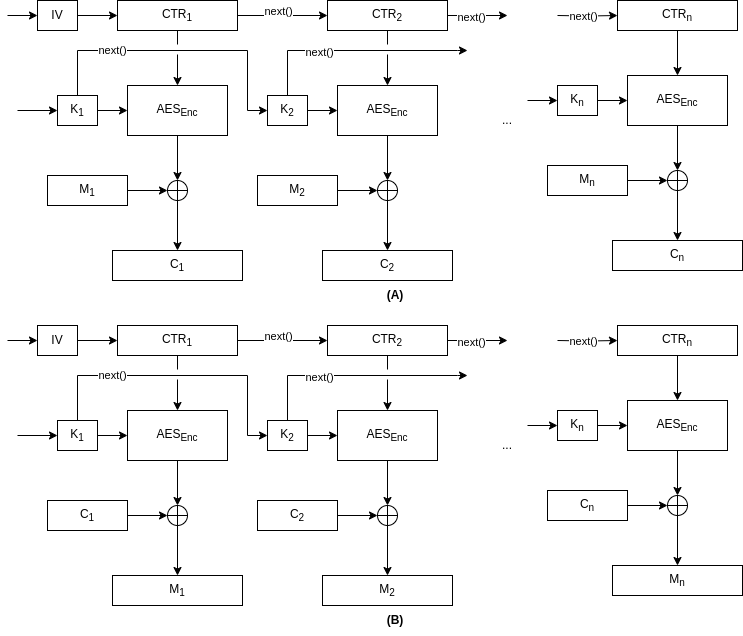
\includegraphics[width=\textwidth]{chapters/res/chapter-3/img/cipher.png}
  \caption{Ilustrasi Sistem Chaos untuk (A) Enkripsi (B) Dekripsi} \label{fig:tls.cipher}
\end{figure}

Nilai $IV$ dan $K1$ keduanya diinisialisasi berdasarkan hasil dari pertukaran kunci. Metode $\text{next}(\cdot)$ merupakan metode untuk memperbaharui sistem chaos berdasarkan persamaan \ref{eq:tls.chaos}. Metode ini dipanggil wajib memenuhi aturan yang telah didefinisikan.

Aturan untuk pembaharuan kunci telah dijelaskan pada bagian III.2.3. Apabila digambarkan, proses pengubahan kunci enkripsi dan MAC dapat dilihat pada gambar \ref{fig:tls.cipher.update.mac.write}. Proses pengubahan kunci dekripsi dan MAC untuk membaca dapat dilihat pada gambar \ref{fig:tls.cipher.update.mac.read}.

\begin{figure}[!h]
  \centering
  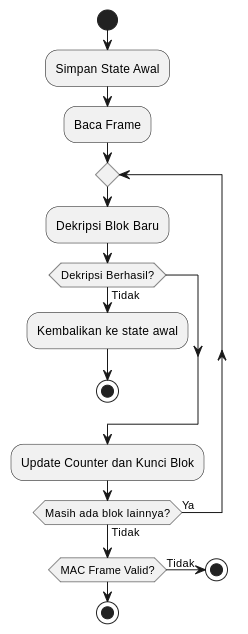
\includegraphics[width=200px]{chapters/res/chapter-3/img/update.write.png}
  \caption{Ilustrasi Proses Pembaharuan Kunci Enkripsi dan MAC pada Proses Penulisan} \label{fig:tls.cipher.update.mac.write}
\end{figure}

Pada proses penulisan, pesan pada mulanya akan dipotong menjadi beberapa frame yang kecil. Setiap frame, pesan akan dilakukan proses \emph{padding} dengan kelipatan 16 bytes. Hal ini agar sesuai dengan panjang blok enkripsi. Setelah pesan dilakukan \emph{padding}, tiap frame akan dilakukan operasi sebagaimana pada gambar \ref{fig:tls.cipher.update.mac.write}. Pesan yang berhasil dienkripsi akan disusun menjadi sebuah \emph{record} yang akan dikirimkan.

\begin{figure}[!h]
  \centering
  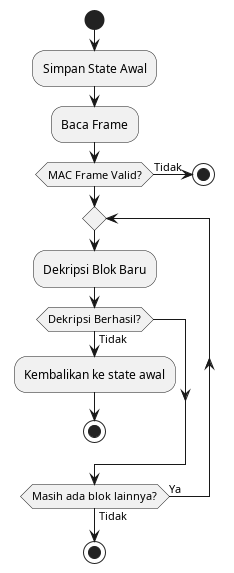
\includegraphics[width=200px]{chapters/res/chapter-3/img/update.read.png}
  \caption{Ilustrasi Proses Pembaharuan Kunci Dekripsi dan MAC pada Proses Pembacaan} \label{fig:tls.cipher.update.mac.read}
\end{figure}

Saat proses pembacaan, pertama-tama frame record harus dipastikan terlebih dahulu MAC valid. Setelah MAC yang diterima valid, maka proses dekripsi akan dilakukan sebagaimana pada gambar \ref{fig:tls.cipher.update.mac.read}. Setelah proses dekripsi berhasil, pesan akan digabungkan dan dilanjutkan ke \emph{layer} yang lebih tinggi. Hash yang digunakan pada MAC adalah SHA-256.

\emph{Cipher} yang dijelaskan pada bagian ini akan ditandai dengan kode \emph{cipher suite} $\text{0xff00}$ pada saat proses \emph{handshake}. Nilai awal $\text{0xff}$ berdasarkan \textcite{rfc5246} merupakan nilai yang privat sehingga dapat dijamin tidak akan bertabrakan dengan \emph{cipher suite} yang telah ada.

\subsection{Spesifikasi \emph{Handshake}}

Proses handshake dilakukan sebagaimana pada protokol TLS yang dijelaskan pada bagian II.10.1. Proses ini dilakukan untuk membangkitkan \emph{master secret} yang digunakan. Terdapat beberapa spesifikasi khusus yang diterapkan pada protokol yang dibangun. Pertukaran kunci yang didukung hanyalah menggunakan Eliptic Curve Diffie-Hellman. Hal ini ditujukan agar keamanan dari \emph{premaster secret} dapat terjamin.

Saat \emph{master secret} berhasil dibangkitkan, perlu dilakukan proses \emph{key expansion}. Panjang kunci yang harus diekspansi adalah 576 bytes. Hal ini dikarenakan diperlukannya tiga pasang sistem \emph{chaos} yang digunakan untuk pembangkitan sistem chaos. Tiap sistem \emph{chaos} memerlukan tiga buah parameter sehingga dibutuhkan 96 bytes per sistem \emph{chaos}.

Persamaan \ref{eq:tls.keyexpansion} menunjukkan proses \emph{key expansion} yang dilakukan. Misalkan $K$ adalah kunci yang diekspansikan sepanjang 576 bytes.

\begin{equation}
  \begin{aligned}
    X_i = f(K[96i:96i+32]) \\
    Y_i = f(K[96i+32:96i+64]) \\
    Z_i = f(K[96i+64:96i+96]) \\
    E_i = (X_i, Y_i, Z_i)
  \end{aligned}
  \label{eq:tls.keyexpansion}
\end{equation}

Tabel \ref{tab:tls.keyexpansion} menunjukan kegunaan dari setiap hasil ekspansi kunci yang dilakukan. Tabel tersebut menjelaskan nilai awal dari sistem \emph{chaos} yang digunakan untuk pembangkitan kunci blok, kunci MAC, dan nilai IV.

\begin{table}[!h]
  \centering
  \caption{Parameter Hasil Ekspansi Kunci} \label{tab:tls.keyexpansion}
  \begin{tabular}{|p{3cm}|p{3cm}|p{6cm}|}
    \hline
    Nama Parameter & Parameter \emph{Chaos} & Deskripsi \\
    \hline
    \emph{MAC Client Key} & $E_1$ & Nilai awal parameter \emph{chaos} yang digunakan client untuk membuat MAC ($H_1$) \\ \hline
    \emph{MAC Server Key} & $E_2$ & Nilai awal parameter \emph{chaos} yang digunakan server untuk membuat MAC ($H_2$) \\ \hline
    \emph{AES Client Key}  & $E_3$ & Nilai awal  parameter \emph{chaos} yang digunakan client untuk melakukan enkripsi ($K_1$) \\ \hline
    \emph{AES Server Key}  & $E_4$ & Nilai awal parameter \emph{chaos} yang digunakan server untuk melakukan enkripsi ($K_1$) \\ \hline
    \emph{IV Client Key}  & $E_5$ & Nilai $IV$ awal yang digunakan client untuk enkripsi \\ \hline
    \emph{IV Server Key}  & $E_6$ & Nilai $IV$ awal yang digunakan server untuk enkripsi \\
    \hline
  \end{tabular}
\end{table}

\subsection{Spesifikasi Pengiriman Pesan}

Pada proses pengiriman pesan, pesan terlebih dahulu harus dipotong menjadi beberapa frame. Setiap frame pesan akan dilakukan proses \emph{padding} dengan kelipatan 16 bytes. Setelah pemasangan padding, akan dilakukan proses enkripsi. Setelah proses enkripsi berhasil, nilai MAC dari proses enkripsi tersebut akan dihitung. Secara matematis, nilai MAC $\text{MAC}_i$ pada frame $i$. dihitung berdasarkan persamaan \ref{eq:tls.mac}.

\begin{equation}
  \begin{aligned}
    \text{MAC}_i = \text{HMAC}_{Hash}(H_i, CB_i) \\
    H_i = \text{next}(H_{i-1}) \\
    H_1 = E_2
  \end{aligned}
  \label{eq:tls.mac}
\end{equation}


Setelah itu, pesan akan disusun menjadi sebuah \emph{record} yang akan dikirimkan. Gambar \ref{fig:tls.application.rec} menunjukkan protokol record yang digunakan untuk mengirimkan pesan.

\begin{figure}[!h]
  \centering
  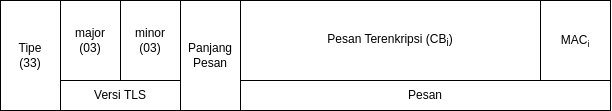
\includegraphics[width=\textwidth]{chapters/res/chapter-3/img/tls.application.record.png}
  \caption{Ilustrasi \emph{Application Record} yang digunakan} \label{fig:tls.application.rec}
\end{figure}

Berdasarkan \textcite{rfc5246}, Nilai tipe haruslah 33. Hal ini menyatakan bahwa pesan yang dikirimkan merupakan \emph{Application Data}. Nilai \emph{version} yang digunakan adalah $\text{0x0303}$. Hal ini menyatakan protokol yang digunakan adalah TLSv1.2. Panjang pesan ($L$) merupakan panjang dari pesan terenkripsi dan MAC. Secara matematis dihitung berdasarkan persamaan \ref{eq:tls.record.length}.

\begin{equation}
  \begin{aligned}
    L = \text{len}(\text{CB}_i\text{ }||\text{ }\text{MAC}_i)
  \end{aligned}
  \label{eq:tls.record.length}
\end{equation}

Pesan terenkripsi merupakan gabungan dari semua blok pesan yang berhasil dienkripsi melalui cipher yang telah dijelaskan sebelumnya.
